\documentclass[crop=false, class=memoir]{standalone}
\usepackage[utf8]{inputenc}%Nødvendig for danske bogstaver
\usepackage[danish]{babel}%Sørger for at ting LaTeX gør automatisk er på dansk
\usepackage{csquotes}
\usepackage{geometry}%Til opsætning af siden
\geometry{lmargin = 2.5cm,rmargin = 2.5cm}%sætter begge magner
\usepackage{lipsum}%Fyldtekst, til brug under test af layoutet
\usepackage{float}
\usepackage{graphicx}%Tillader grafik
\usepackage{epstopdf}%Tillader eps filer
\usepackage{marginnote}% Noter i margen
\interfootnotelinepenalty=10000 %undgår at fodnoter bliver spilittet op.
\usepackage[sorting=none]{biblatex}
\addbibresource{litteratur.bib}
\usepackage[hidelinks]{hyperref}%Tillader links
\usepackage{subcaption} % Tillader underfigurer
\usepackage[font={small,sl}]{caption}	% Caption med skrå tekst ikke kursiv

\usepackage{xcolor} %Bruges til farver
\usepackage{forloop} %Bruges til nemmere for loops

\newcounter{opgave}[chapter] %Definerer opgavenumrene og hvornår de nulstilles
\renewcommand{\theopgave}{\thechapter.\arabic{opgave}} %Definerer udseende af opgavenummereringen
\newcounter{delopgave}[opgave] %Definerer delopgavenumrene
\newcounter{lvl} %Definerer en "variabel" til senere brug

\definecolor{markerColor}{rgb}{0.0745098039, 0.262745098, 0.584313725} %Definerer farven af markøren
\newcommand{\markerSymbol}{\ensuremath{\bullet}} %Definerer tegnet for markøren
\newlength{\markerLength} %Definerer en ny længde
\settowidth{\markerLength}{\markerSymbol} %Sætter den nye længde til bredden af markøren

\newenvironment{opgave}[2][0]{%Definerer det nye enviroment, hvor sværhedsgraden er den første parameter med en default på 0
\newcommand{\opg}{\refstepcounter{delopgave}\par\vspace{0.1cm}\noindent\textbf{\thedelopgave)\space}}%Definerer kommando til delopgave
\refstepcounter{opgave}%Forøger opgavenummer med 1 og gør den mulig at referere til
\setcounter{lvl}{#1}%Sætter "variablen" lvl lig med angivelsen af sværhedsgraden
\noindent\hspace*{-0.75em}\hspace*{-\value{lvl}\markerLength}\forloop{lvl}{0}{\value{lvl}<#1}{{\color{markerColor}\markerSymbol}}\hspace*{0.75em}%Sætter et antal af markører svarende til sværhedsgraden
\textbf{Opgave \theopgave : #2}\newline\nopagebreak\ignorespaces}{\bigskip} %Angiver udseende af titlen på opgaverne samt mellemrummet mellem opgaver



\usepackage{mathtools}%Værktøjer til at skrive ligninger
\renewcommand{\phi}{\varphi}%Vi bruger varphi
\renewcommand{\epsilon}{\varepsilon}%Vi bruger varepsilon
\usepackage{physics}%En samling matematikmakroer til brug i fysiske ligninger
\usepackage{braket}%Simplere kommandoer til bra-ket-notation
\usepackage{siunitx}%Pakke der håndterer SI enheder godt
\DeclareSIUnit\clight{\text{\ensuremath{c}}} % Lysets fart i vakuum som c og ikke c_0
\usepackage{chemmacros}
\usechemmodule{isotopes}
\usepackage{tikz}
\usepackage[danish]{cleveref}
\usepackage{nicefrac}
% \renewcommand{\ref}[1]{\cref{#1}}
\creflabelformat{equation}{#2(#1)#3}
\crefrangelabelformat{equation}{#3(#1)#4 to #5(#2)#6}
\crefname{equation}{ligning}{ligningerne}
\Crefname{equation}{Ligning}{Ligningerne}
\crefname{section}{afsnit}{afsnitene}
\Crefname{section}{Afsnit}{Afsnitene}
\crefname{figure}{figur}{figurene}
\Crefname{figure}{Figur}{Figurene}
\crefname{table}{tabel}{tabellerne}
\Crefname{table}{Tabel}{Tabellerne}
\crefname{opgave}{opgave}{opgaverne}
\Crefname{opgave}{Opgave}{Opgaverne}
\crefname{delopgave}{delopgave}{delopgaverne}
\Crefname{delopgave}{Delopgave}{Delopgaverne}

\newcommand{\eqbox}[1]{\begin{empheq}[box=\fbox]{align}
	\begin{split}
	#1
	\end{split}
\end{empheq}}

\newcommand{\kb}{\ensuremath{k_\textsc{b}}}

\DeclareSIUnit{\parsec}{pc}
\DeclareSIUnit{\lightyear}{ly}
\DeclareSIUnit{\astronomicalunit}{AU}
\DeclareSIUnit{\year}{yr}
\DeclareSIUnit{\solarmass}{M_\odot}
\DeclareSIUnit{\solarradius}{R_\odot}
\DeclareSIUnit{\solarluminosity}{L_\odot}
\DeclareSIUnit{\solartemperature}{T_\odot}
\DeclareSIUnit{\earthmass}{M_\oplus}
\DeclareSIUnit{\earthradius}{R_\oplus}
\DeclareSIUnit{\jupitermass}{M_J}

% Infobokse og lignende
% http://mirrors.dotsrc.org/ctan/graphics/awesomebox/awesomebox.pdf
% \usepackage{awesomebox}


% Egen infobokse (virker kun med begrænsede symboler)

\usepackage[framemethod=tikz]{mdframed}
\usetikzlibrary{calc}
\usepackage{kantlipsum}

\usepackage[tikz]{bclogo}

\tikzset{
    % lampsymbol/.style={scale=2,overlay}
    % lampsymbol/.pic={\centering\tikz[scale=5]\node[scale=10,rotate=30]{\bclampe}}.style={scale=2,overlay}
    infosymbol/.style={scale=2,overlay}
}

\newmdenv[
    hidealllines=true,
    nobreak,
    middlelinewidth=.8pt,
    backgroundcolor=blue!10,
    frametitlefont=\bfseries,
    leftmargin=.3cm, rightmargin=.3cm, innerleftmargin=2cm,
    roundcorner=5pt,
    % skipabove=\topsep,skipbelow=\topsep,
    singleextra={\path let \p1=(P), \p2=(O) in ($(\x2,0)+0.92*(1.1,\y1)$) node[infosymbol] {\bcinfo};},
    % singleextra={\path let \p1=(P), \p2=(O) in ($(\x2,0)+0.5*(2,\y1)$) node[infosymbol] {\bcinfo};},
]{info}

% Skal bruges som
% \begin{info}[frametitle={Titel}]
%     Tekst
% \end{info}
\usepackage{import}
\begin{document}
\chapter{Elektromagnetisme} \label{chap:elektro_facit}

\begin{opgave}{Coulombkraften}
    \opg Indsættes de opgivne tal fås
    \begin{enumerate}
        \item $F = \dfrac{1}{4\pi\epsilon_0}\dfrac{q_1q_2}{r^2} = \SI{8.99e9}{\newton} = \SI{8.99}{\giga\newton}$.
        \item $F = \dfrac{1}{4\pi\epsilon_0}\dfrac{q_1q_2}{r^2} = -\SI{8.99e9}{\newton} = -\SI{8.99}{\giga\newton}$.
        \item $F = \dfrac{1}{4\pi\epsilon_0}\dfrac{q_1q_2}{r^2} = \SI{18.0e9}{\newton} = \SI{18.0}{\giga\newton}$.
        \item $F = \dfrac{1}{4\pi\epsilon_0}\dfrac{q_1q_2}{r^2} = \SI{2.25e9}{\newton} = \SI{2.25}{\giga\newton}$.
    \end{enumerate}
    \[ \]
    \opg Når den ene ladning skifter fortegn, så skifter kraften også fortegn. Fordobles størrelsen af den ene ladning, så fordobles størrelsen af kraften.
    \[ q_1\to -2q_1 \]
    Derudover bliver ladningernes indbyrdes afstand fordoblet.
    \[ r\to 2r\]
    Så vi har at kraften bliver
    \[ F=\frac{1}{4\pi\varepsilon_0}\frac{q_1q_2}{r^2}\to\frac{1}{4\pi\varepsilon_0}\frac{(-2q_1)q_2}{(2r)^2}=-\frac{1}{2}F.\]
    Kraften bliver dermed halvt så stor og skifter retning.
    \opg Vi skal bruge tilfælde 1. fra delopgave 1).
    \[ F=\SI{8.99e9}{\newton} \]
    Her er $m_1=\SI{1.00}{\kilo\gram}$ og $m_2=\SI{2.00}{\kilo\gram}$.
    Accelerationen på de to ladninger er
    \[ a_1 = \dfrac{F}{m_1} = \dfrac{1}{4\pi\epsilon_0}\dfrac{q_1q_2}{m_1r^2} = \SI{8.99e9}{\metre\per\second\squared} \]
    og
    \[ a_2 = \dfrac{F}{m_1} = \dfrac{1}{4\pi\epsilon_0}\dfrac{q_1q_2}{m_2r^2} = \SI{4.49e9}{\metre\per\second\squared}\]
    Her accelererer væk fra hinanden.
    \opg Her fås
    %
    \begin{enumerate}
        \setcounter{enumi}{1}
        \item $a_1 = \dfrac{F}{m_1} = \dfrac{1}{4\pi\epsilon_0}\dfrac{q_1q_2}{m_1r^2} = -\SI{8.99e9}{\metre\per\second\squared} = -\SI{8.99}{\giga\metre\per\second\squared}$.
        \item $a_1 = \dfrac{F}{m_1} = \dfrac{1}{4\pi\epsilon_0}\dfrac{q_1q_2}{m_1r^2} = \SI{18.0e9}{\metre\per\second\squared} = \SI{18.0}{\giga\metre\per\second\squared}$.
        \item $a_1 = \dfrac{F}{m_1} = \dfrac{1}{4\pi\epsilon_0}\dfrac{q_1q_2}{m_1r^2} = \SI{2.25e9}{\metre\per\second\squared} = \SI{2.25}{\giga\metre\per\second\squared}$.
    \end{enumerate}
    I 2. accelererer ladningerne mod hinanden, og væk fra hinanden i 3. og 4.
    \opg Da $m_2 = 2m_1$ accelereres ladning $1$ dobbelt så hurtigt som ladning $2$ uanset hvad kraften er. I tilfælde $1$, $3$ og $4$ har ladningerne samme fortegn, hvorfor de frastøder hinanden og dermed bevæger sig væk fra hinanden. Forskellen på tilfælde $1$ og $3$ er størrelsen på ladningen. Bevægelserne ser derfor ens ud, men alting går dobbelt så hurtigt i tilfælde $3$ som i tilfælde $1$. I tilfælde $4$ starter ladningerne dobbelt så langt fra hinanden som i tilfælde $1$. Selve bevægelsen vil stadig være ens, da det er den samme kraft i begge tilfælde. Alting vil dog gå $1/4$ så langsomt. I disse tre tilfælde vil ladningerne bevæge sig hurtigere og hurtigere væk fra hinanden og forsvinde uendeligt langt væk fra hinanden. Deres acceleration vil dog blive mindre og mindre. I tilfælde $2$ vil de to ladninger tiltrække hinanden, hvorfor de vil bevæge sig tættere og tættere på hinanden. Kraften på dem vil hele tiden øges, hvor accelerationen hele tid stiger. I et kort tidsrum efter de to ladninger frigives vil størrelserne på hastighederne i tilfælde $1$ og $2$ minde om hinanden, men dette holder op med at være tilfældet, når ladningernes indbyrdes afstand har ændret sig betydeligt fra udgangspunktet.
\end{opgave}

\begin{opgave}{Tre ladninger på en linje}
    \opg Hver ladning bidrager med henholdsvis:
    \begin{align}
        \va{F}_1=\frac{1}{4\pi\epsilon_0}\frac{qQ(x-a)}{|x-a|^3}\vu{x}\qquad \qquad \va{F}_2=\frac{1}{4\pi\epsilon_0}\frac{qQ(x+a)}{|x+a|^3}\vu{x}
    \end{align}
    Lægges de to krafter sammen, fås
    \begin{align}
        \va{F}=\frac{qQ}{4\pi\epsilon_0}\left(\frac{(x-a)}{|x-a|^3}+\frac{(x+a)}{|x+a|^3}\right)\vu{x}
    \end{align}
    \opg
    \begin{figure}[H]
        \centering
        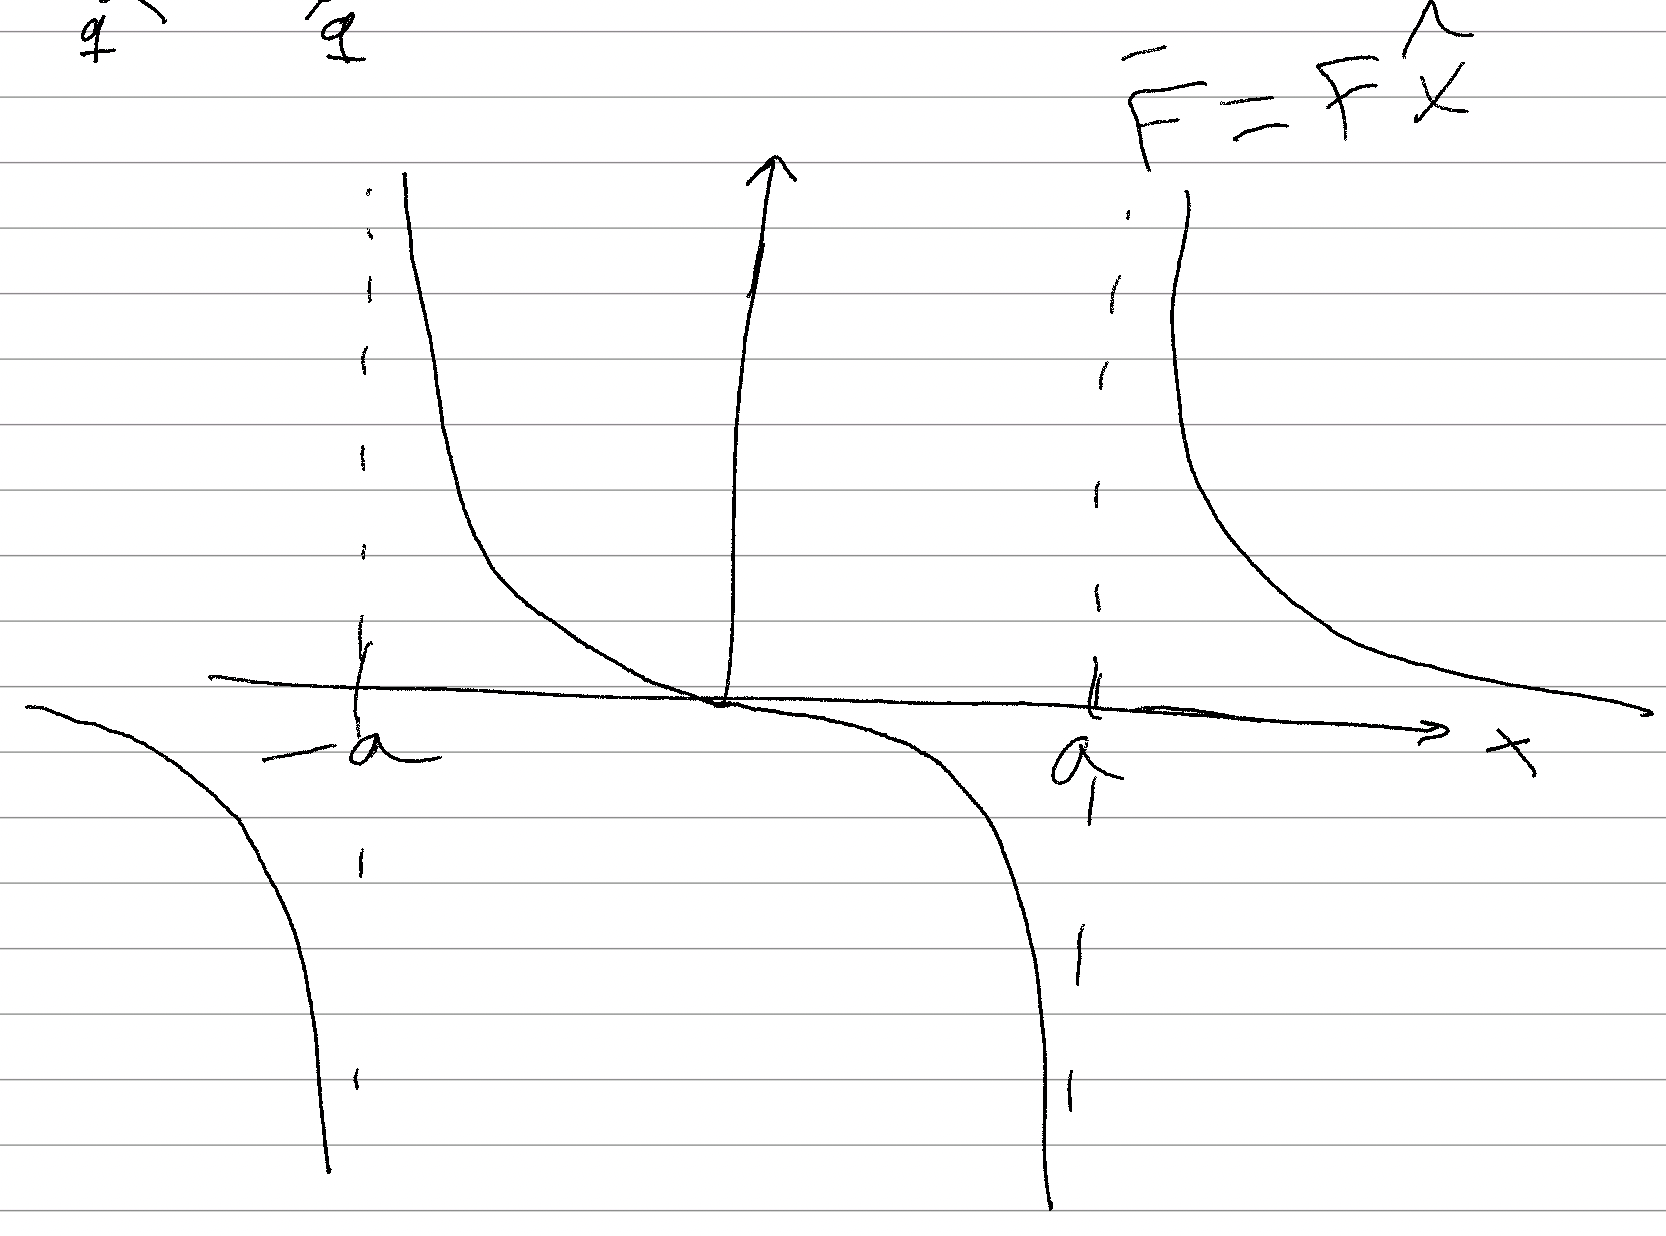
\includegraphics[width=0.8\textwidth]{Elektro/Elekfig/elektro_opg4,2.png}
    \end{figure}
    \opg Ved $x=0$ så er $F=0$, så ladningen $q$ står stille.
    \opg For $x\gg a$ bliver
    \begin{align*}
        \va{F}&=\frac{Qq}{4\pi\epsilon_0}\left(\frac{(x-a)}{|x-a|^3}+\frac{(x+a)}{|x+a|^3}\right)\vu{x}\\
        &\approx \frac{Qq}{4\pi\epsilon_0}\left(\frac{x}{x^3}+\frac{x}{x^3}\right)\vu{x}\\
        &=\frac{(2q)Q}{4\pi\varepsilon_0}\frac{1}{x^2}\vu{x},
    \end{align*}
    hvilket er kraften på en ladning $Q$ pga. en ladning $2q$ placeret ved $x=0$. Når man er langt væk, kan man nemlig betragte begge $+q$ ladninger som værende én samlet ladning.
\end{opgave}

\begin{opgave}{Firkant konfiguration}
Se billedet:
\begin{figure}
    \centering
    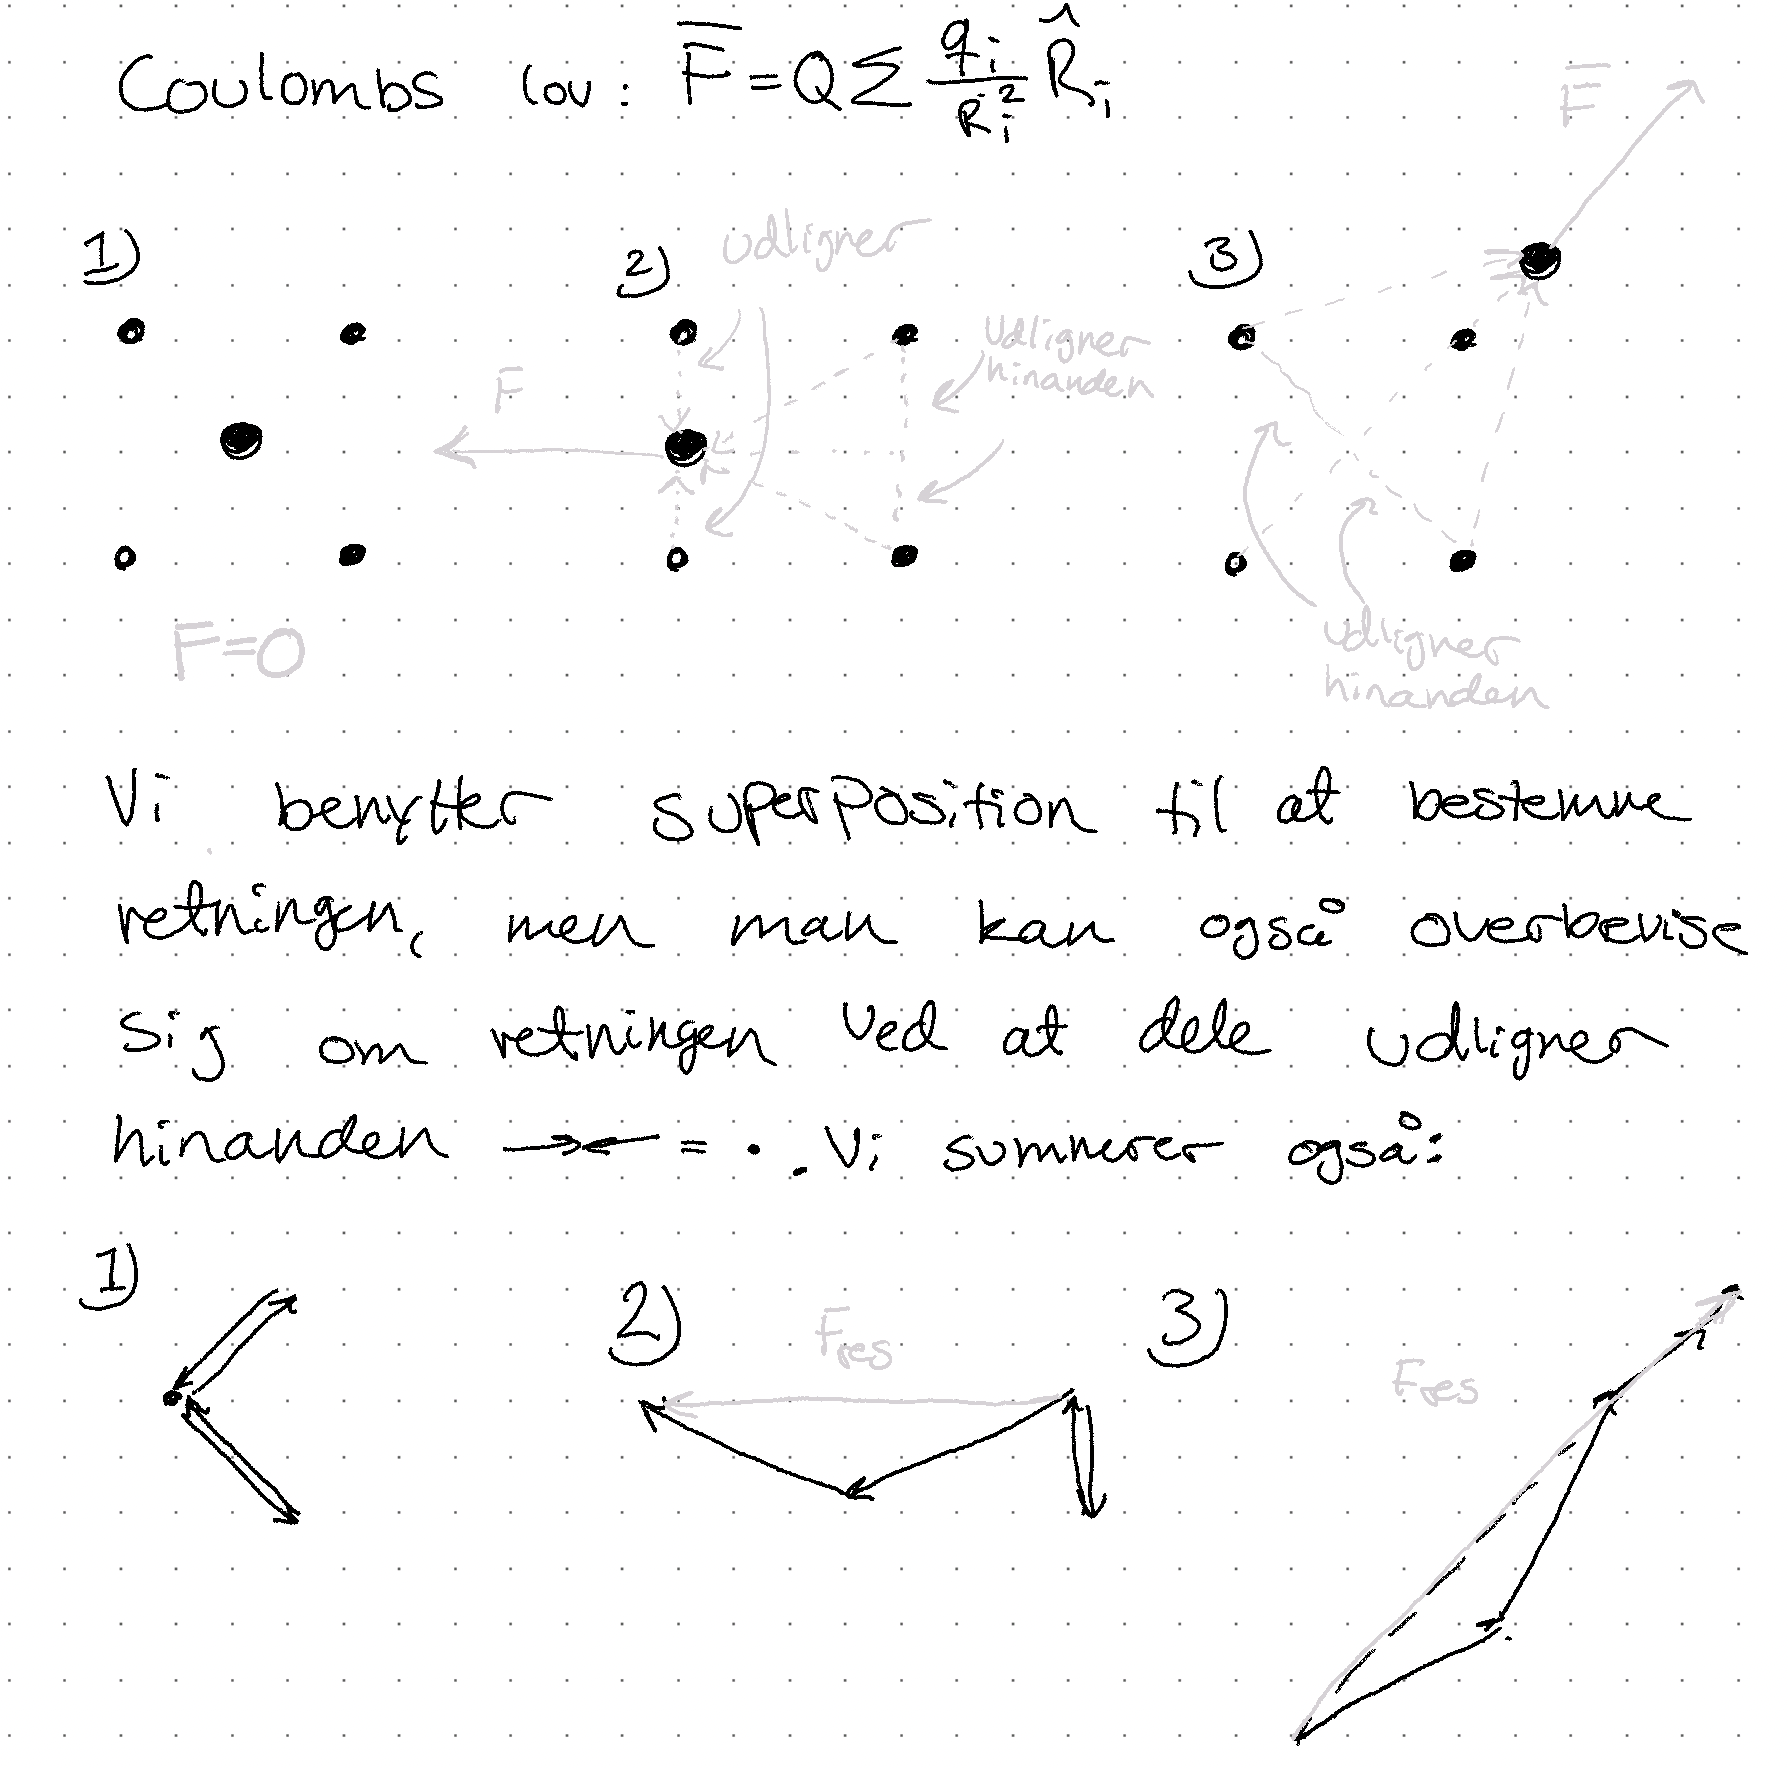
\includegraphics[width=\textwidth]{Elektro/Elekfig/elektro_opg4,3.png}
    \caption{}
    \label{fig:my_label}
\end{figure}


\end{opgave}
\begin{opgave}{Fluxopgave I}
    \opg
    Vi har, at fluxen er
    \begin{align*}
    \oint\va{E}\cdot\va{\dd{a}}=\int_1\va{E}\cdot\va{\dd{a}}+\int_2\va{E}\cdot\va{\dd{a}}+\int_3\va{E}\cdot\va{\dd{a}}
    \end{align*}
    Hvor fladerne 1 og 2, er cirkeloverfladerne på enderne af cylinderne og flade 3 er den resterende overflade (Den der krummer). Men for flade 1 og 2 er $\va{E}\cdot\va{\dd{a}}=0$, og for flade 3 har vi.
    \begin{align}
        \int_3(\frac{\lambda}{2\pi r\epsilon_0}\vu{s})\cdot(\dd{a}\vu{s})=\int_3\frac{\lambda}{2\pi r \epsilon_0}\dd{a}
    \end{align}
    Men på overfladen 3 er E-feltet konstant og er lig med $|E|(R)=\frac{\lambda}{2\pi R\epsilon_0}$ (Altså, $|E|(R)$, er E-feltets størrelse i $r=R$). Så vi har, at integralet bliver:
    \begin{align*}
        |E|(R)\int_3\dd{a}=\frac{\lambda}{2\pi R\epsilon_0}\int_3\dd{a}
    \end{align*}
    Fladen 3 er $\int\dd{a}=2\pi R L$, da er fluxen
    \begin{align*}
        \oint\va{E}\cdot\va{\dd{a}}=\frac{\lambda}{2\pi R \epsilon_0}2\pi RL=\frac{\lambda L}{\epsilon_0}
    \end{align*}
    
    \opg
    Nu er overfladen af cylinderen (minus enderne) $\int\dd{a}=2\pi (2R)L$, og E-feltet i 2R er $|E|(2R)=\frac{\lambda}{2\pi(2R)\epsilon_0}$
    Så fluxen bliver
    \begin{align*}
        |E|(2R)\int_3\dd{a}=\frac{\lambda}{2\pi (2R)}2\pi (2R)L=\frac{\lambda L}{\epsilon_0}
    \end{align*}
    \opg
    Denne gang er flade 3 $\int\dd{a}=2\pi R(2L)$, og størrelsen af E-feltet er bare $|E|(R)$. Fluxen er dermed:
    \begin{align*}
        |E|(R)\int_3\dd{a}=\frac{\lambda}{2\pi R \epsilon_0}2\pi R (2L)=\frac{2\lambda L}{\epsilon_0}
    \end{align*}
    \opg Fluxen er dobbelt så stor i 3) end i 1) og 2), da vi har indlukket dobbelt så meget ladning! $2\lambda L$ ladning fremfor $\lambda L$ ladning.
\end{opgave}

\begin{opgave}{Fluxopgave II}
    \opg
    E-feltet for hver plade summeres sammen, og bliver 
    \begin{align*}
        \va{E}=\frac{\sigma}{\epsilon_0}\vu{n}
    \end{align*}
    Hvor $\vu{n}$ er en vektor der peger op over begge plade, ned under pegge plader og er 0 i mellem pladerne. Hvis $\vu{z}$ peger op, så kan $\vu{n}$ også skrives som:
    \begin{align*}
        \vu{n}=\begin{cases} 
      \frac{\sigma}{\epsilon_0}\vu{z} & \textit{Over begge plader} \\
      0 & \textit{I mellem begge plader} \\
      -\frac{\sigma}{\epsilon_0}\vu{z} & \textit{Under begge plader}
   \end{cases}
    \end{align*}
    \opg
    Helt generelt kan overfladen deles op i 6. Da er fluxen:
    \begin{align*}
        \oint\va{E}\cdot\va{\dd{a}}=\int_{over}\va{E}\cdot\va{\dd{a}}+\int_{under}\va{E}\cdot\va{\dd{a}}+\int_1\va{E}\cdot\va{\dd{a}}+\int_2\va{E}\cdot\va{\dd{a}}+\int_3\va{E}\cdot\va{\dd{a}}+\int_4\va{E}\cdot\va{\dd{a}}
    \end{align*}
    Men $\va{E}\cdot\va{\dd{a}}=0$ for fire af overfladerne, så vi har tilbage:
    \begin{align*}
        \oint\va{E}\cdot\va{\dd{a}}=\int_{over}\va{E}\cdot\va{\dd{a}}+\int_{under}\va{E}\cdot\va{\dd{a}}
    \end{align*}
    Men $\va{E}$ er nul på fladen under (E-feltet er nul mellem pladerne), så tilbage er kun overfladen over.
    \begin{align*}
        \oint\va{E}\cdot\va{\dd{a}}=\int_{over}\va{E}\cdot\va{\dd{a}}=\int_{under}\frac{\sigma}{\epsilon_0}\dd{a}=\frac{\sigma A}{\epsilon_0}
    \end{align*}
    \opg
    Igen er det kun overfladerne over og under, der kan give noget. Denne gang bidrager begge overflader med det samme (E-feltet har samme styrke under og over begge plade). Derudover er $\va{E}\cdot\va{\dd{a}}=|E|\dd{a}$ for begge overflader. Dermed får vi:
    \begin{align*}
        \oint\va{E}\cdot\va{\dd{a}}=\int_{over}\va{E}\cdot\va{\dd{a}}+\int_{under}\va{E}\cdot\va{\dd{a}}=\frac{\sigma A}{\epsilon_0}+\frac{\sigma A}{\epsilon_0}=\frac{2\sigma A}{\epsilon_0}
    \end{align*}
    \opg
    Fluxen er dobbelt så stor i 2) end i 1), da vi har indlukket dobbelt så meget ladning ($2A\sigma$ fremfor $A\sigma$).
    
\end{opgave}

\begin{opgave}
    \opg
    Vi betragter en linjeladning $\lambda$ og placerer Q et tilfældig sted distancen $r$ (vinkelret distance) væk fra linjeladning. Da vil Q danne en vinkel $\theta$ med linjeladningen. Hvis vi bibeholder distancen r og varierer $\theta$, således vi kommer hele vejen rundt (altså $\theta$ varierer fra 0 til 360 grader), så vil Q for hvert $\theta$ skubbes vinkelret væk fra linjeladningen. Da Q's position er tilfældig, så gælder dette overalt i rummet. Se figur \ref{em:opg:4,6}
    \begin{figure}
        \centering
        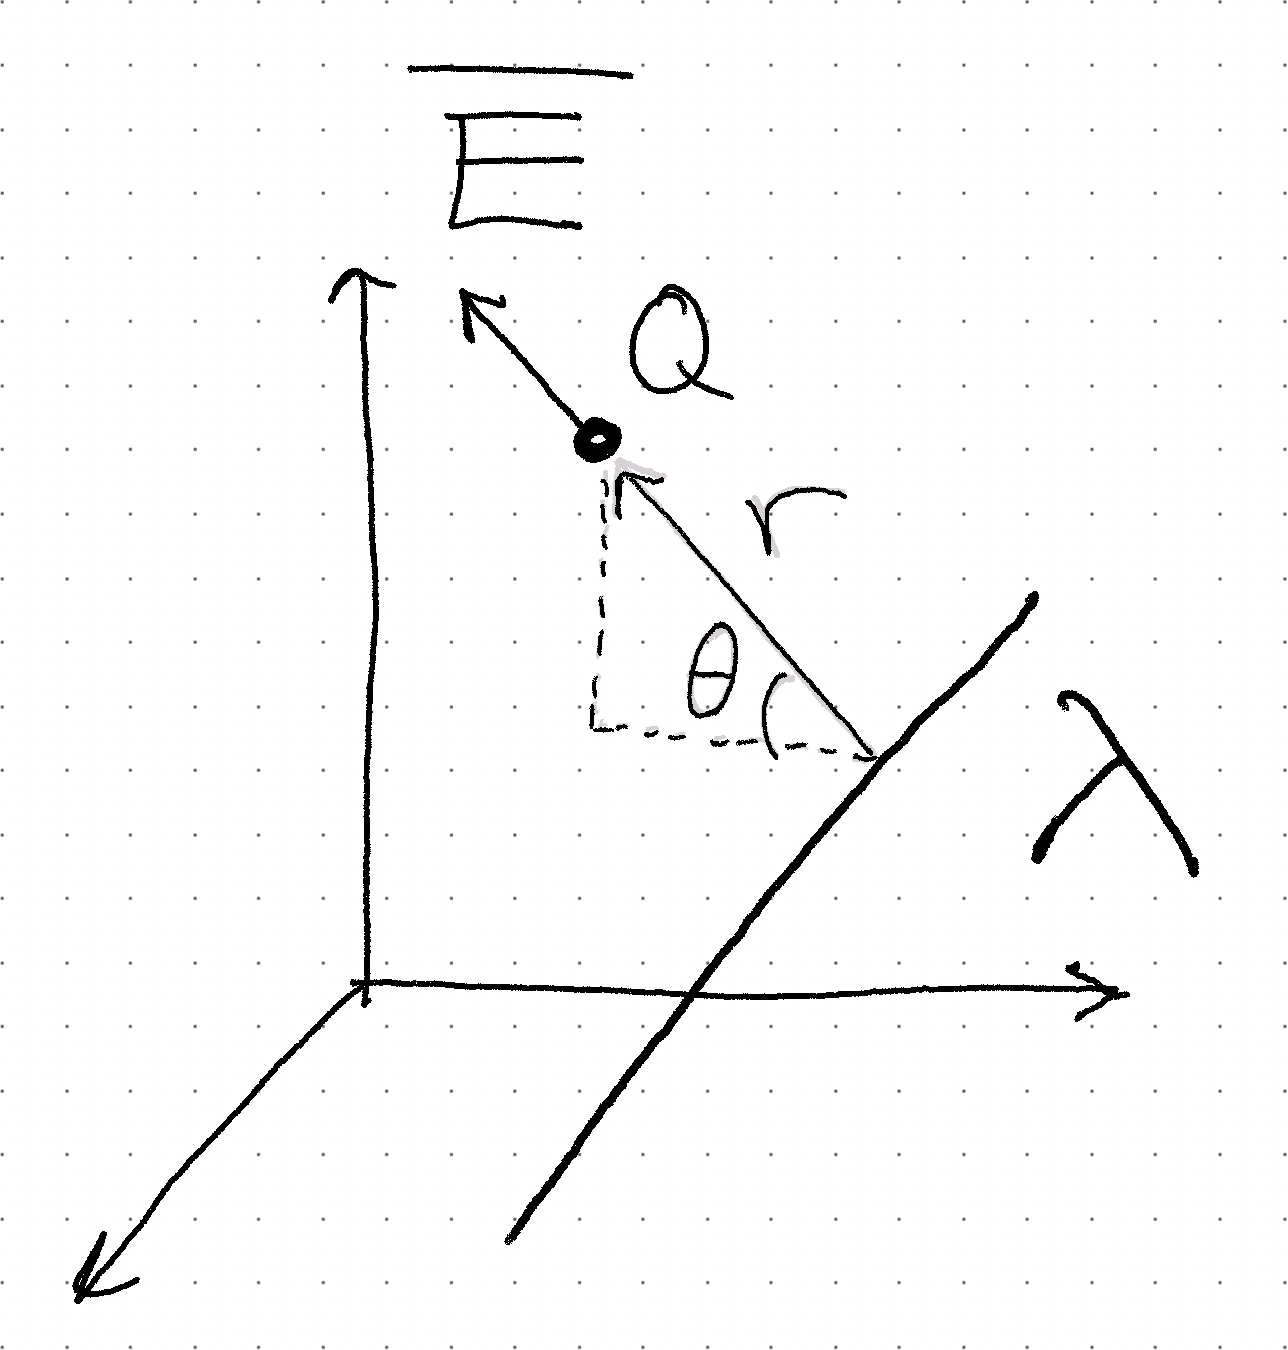
\includegraphics[scale=0.3]{Elektro/Elekfig/4.6.png}
        \caption{}
        \label{em:opg:4,6}
    \end{figure}
    \opg
    E-feltet er rotationssymmetrisk, da hvis man varierer $\theta$, og beholder distancen r, så har den fysiske situation ikke ændret sig. Derfor må E-feltet være det samme ved en ændring af $\theta$
    \opg
    Hvis vi vælger en cylinderoverflade, så vil enderne af cylinderen resulterer i, at $\va{E}\cdot\va{\dd{a}}=0$, mens for den krumme cylinder overflade får vi $\va{E}\cdot\va{\dd{a}}=|E|\dd{a}$.
    \opg
    Vi har
    \begin{align*}
        \oint \va E \cdot \dd{\va a} = \int_{S_1} \va E \cdot \dd{\va a} + \int_{S_2} \va E \cdot \dd{\va a} + \int_{S_3} \va E \cdot \dd{\va a}=\int_{S_1}|E|\dd{a}
    \end{align*}
    Men da |E| er uændret langs den krumme overflade, så kan vi trække den udenfor integralet. Vi ved også overfladen af cylinderen er $2\pi r L$. Vi får altså
    \begin{align*}
        \oint \va E \cdot \dd{\va a} =\int_{S_1}|E|\dd{a}=|E|\int_{S_1}\dd{a}=|E|2\pi r L
    \end{align*}
    \opg
    Gauss lov siger:
    \begin{align*}
        \oint \va E \cdot \dd{\va a}=\frac{Q_enc}{\epsilon_0}
    \end{align*}
    Hvor $Q_{enc}=\lambda L$. Dermed fås
    \begin{align*}
        |E|2\pi r L=\frac{\lambda L}{\epsilon_0} \qquad \xrightarrow{} |E|=\frac{\lambda}{2\pi r \epsilon_0}
    \end{align*}
    Og da $\va{E}=|E|\vu{s}$, så bliver E-feltet endeligt:
    \begin{align*}
        \va{E}=\frac{\lambda}{2\pi r \epsilon_0}\vu{s}
    \end{align*}
\end{opgave}
\begin{opgave}{Ladet kugle}
    \opg
    Vi benytter, at en hul sfære overflade med radius $R_0$ og overfladesladning $\sigma$ udspænder et E-felt givet ved $\va{E}=\frac{1}{4\pi\epsilon_0}\frac{1}{r^2}\vu{r}$ for $r>R$, og at det er $0$ for $r<R$ (eksemplet gennemgået i sfærisk symmetrisk E-felt afsnittet). Vi kan dernæst bestemme os for at konstruere den solide kugle fra sfære overflader. Hvis vi kigger på E-feltet for $r>R$ ($R$ er radius af den solide kugle), så vil hver sfære overflade bidrager med en radiel påvirkning, og da vil E-feltet være radielt. For $r<R$, så vil alle overflader der opfylder $r<R_0$ bidrage med ingenting (E-feltet er nul). Mens de overflader der opfylder $r>R_0$ igen bidrage med et parallelt E-felt. Vi har altså, at $\va{E}=|E|\vu{r}$ (og $\va{\dd{a}}=\dd{a}\vu{r}$)
    \opg
    Bruger vi en sfære overflade med radius r centeret i origo som gauss overflade, så har vi:
    \begin{align*}
        \oint\va{E}\cdot\va{\dd{a}}=\int|E|\dd{a}=|E|\int\dd{a}=\frac{Q_{enc}}{\epsilon_0}
    \end{align*}
    Og overfladen af sfæren er $\int\dd{a}=4\pi r^2$. Dermed får vi, at:
    \begin{align*}
        |E|=\frac{Q_{enc}}{4\pi \epsilon_0}\frac{1}{r^2}
    \end{align*}
    Og
    \begin{align*}
        \va{E}=\frac{Q_{enc}}{4\pi \epsilon_0}\frac{1}{r^2}\vu{r}
    \end{align*}
    Man kan også indsætte, at $Q_{enc}=\frac{4}{3}\pi R^3\rho$. Men da det er en konstant, så er det ikke så interessant for opførelsen af feltet.
    \opg
    Vi vælger igen en sfære overflade med radius r centeret i origo. Alt udregning bliver det samme til og med størrelsen af E-feltet, men denne gang er $Q_{enc}=\frac{4}{3}\pi r^3\rho$, hvilken har en effekt på opførelsen af E-feltet.
    \begin{align*}
        |E|=\frac{Q_{enc}}{4\pi \epsilon_0}\frac{1}{r^2}=\frac{4/3\pi r^3\rho}{4\pi \epsilon_0}\frac{1}{r^2}=\frac{\rho}{3\epsilon_0}r
    \end{align*}
    og
    \begin{align*}
        \va{E}=\frac{\rho}{3\epsilon_0}r\vu{r}
    \end{align*}
\end{opgave}
\begin{opgave}{Cylinder ladningskonfigurationer}
    \opg
    For at anskue hvordan E-feltet peger, så splitter vi cylinderen op i uendelige linjeladninger $\lambda$. Vi betrager dernæst et 2D perspektiv som vist i fig \ref{em:opg:4.8}. Da kan man se, at man kan parvis betragte to linjeladninger og at deres bidrag summeret sammen resulterer i, at E-feltet peger radielt ud fra centrum. Dette kan vi gentage for alle linjeladninger, og det resulterende E-felt peger radielt ud fra cirkeltværsnittet (Dette er også sammen retning som $\vu{s}$ vektoren, som vi har set tidligere).
    \begin{figure}
        \centering
        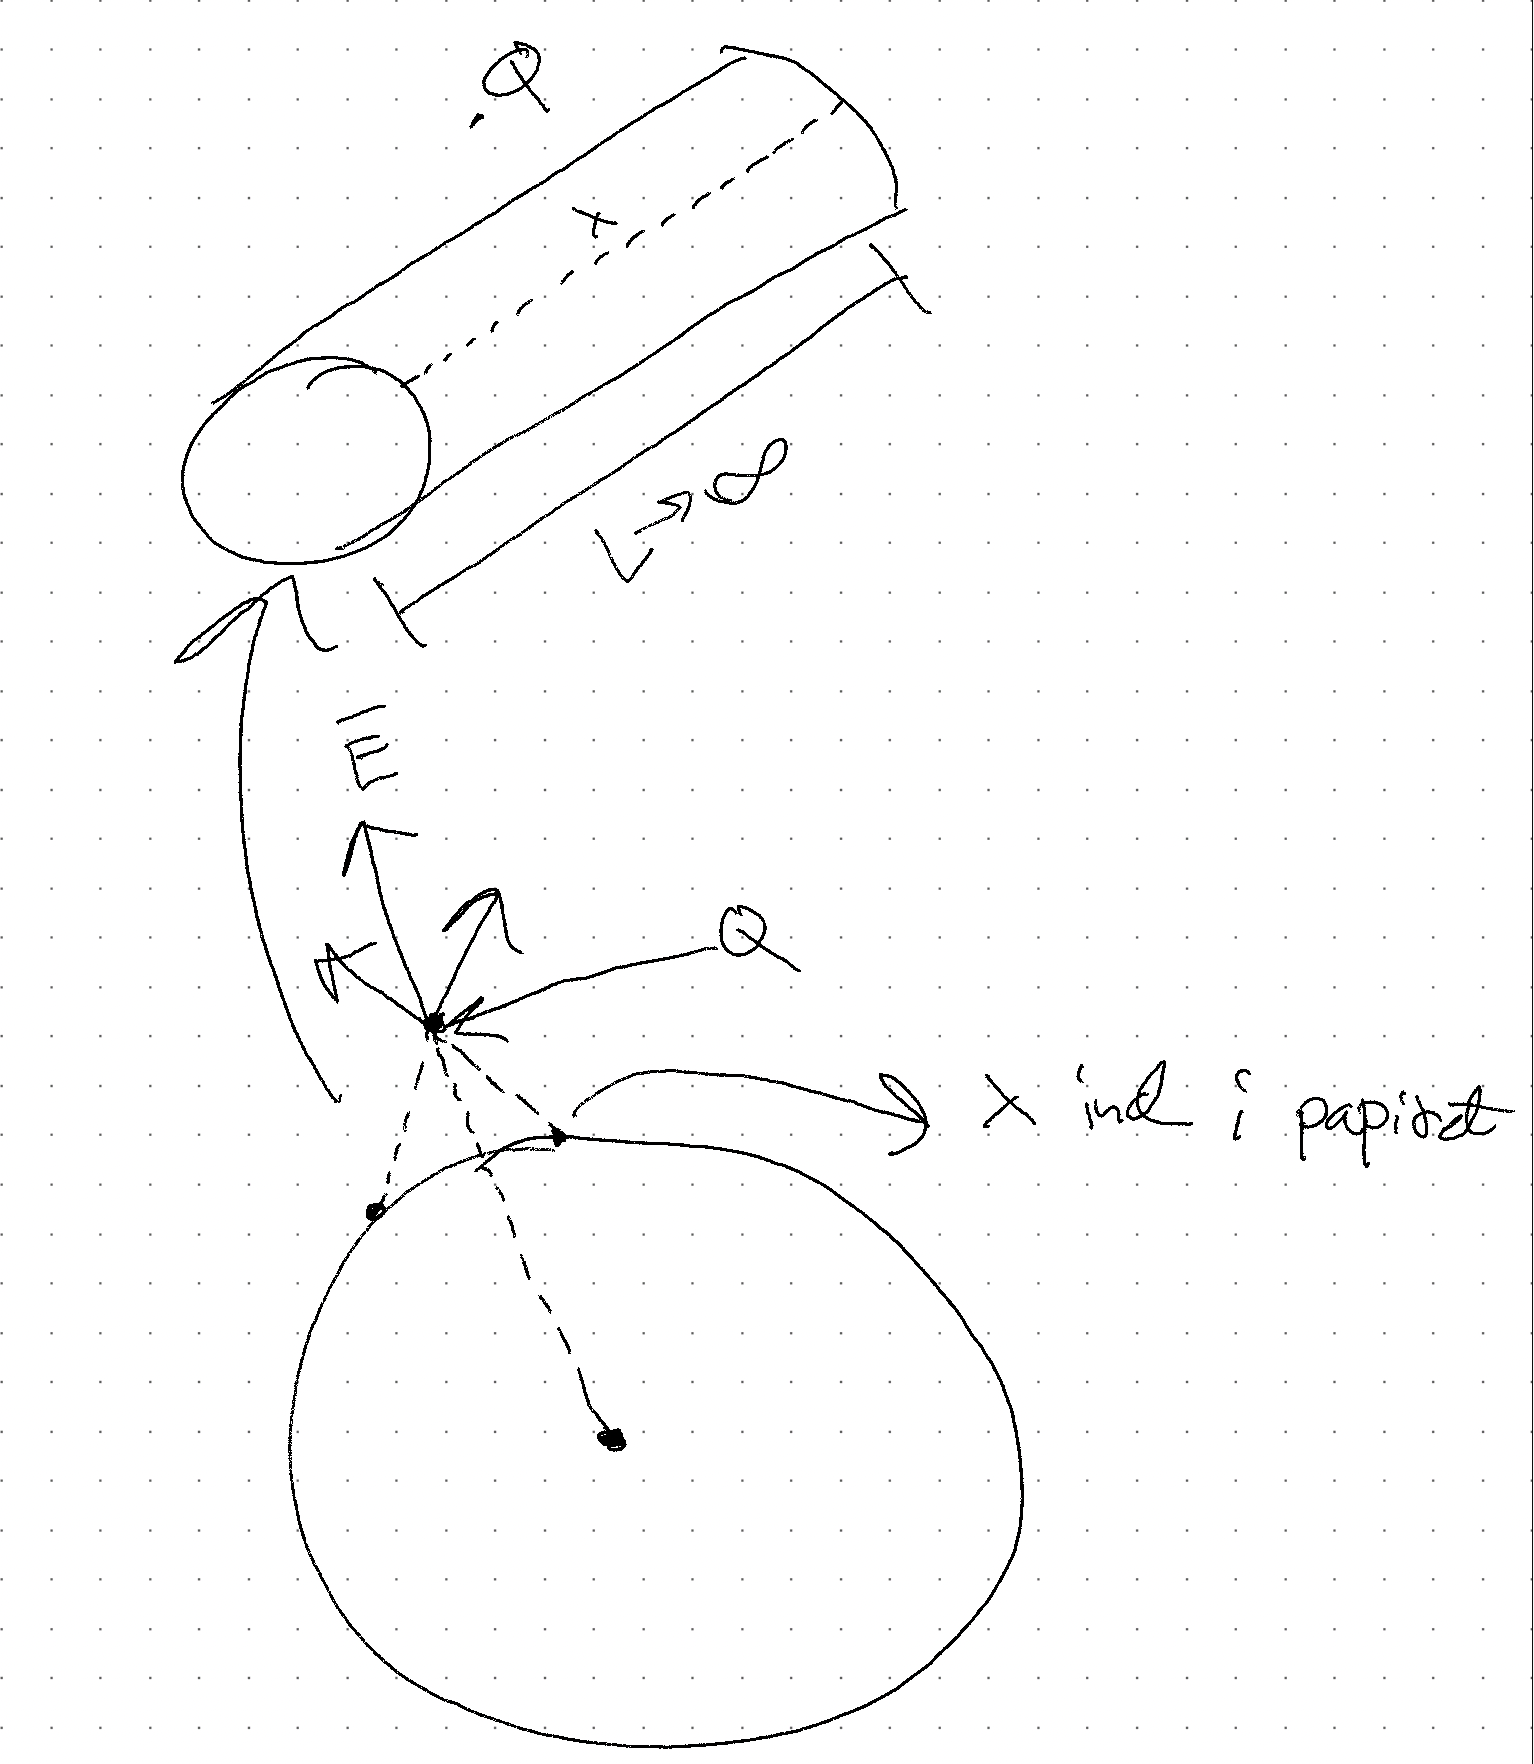
\includegraphics[scale=0.4]{Elektro/Elekfig/4.8.png}
        \caption{}
        \label{em:opg:4.8}
    \end{figure}
    \opg
    Vi vælger en cylinder gauss overflade, og da $\va{E}=|E|\vu{s}$, så kan vi gentage meget af det vi har lavet i de andre opgaver.
    \begin{align*}
        \oint\va{E}\cdot\va{\dd{a}}=\int_1\va{E}\cdot\va{\dd{a}}+\int_2\va{E}\cdot\va{\dd{a}}+\int_3\va{E}\cdot\va{\dd{a}}=\int_{S_1}|E|\dd{a}=|E|\int_{S_1}\dd{a}=|E|2\pi r L=
    \end{align*}
    Anvender vi også gauss lov $\oint\va{E}\cdot\va{\dd{a}}=\frac{Q_{enc}}{\epsilon_0}$ og $Q_{enc}=\sigma2\pi R L$, så får vi relationen:
    \begin{align*}
        |E|2\pi r L=\frac{Q_{enc}}{\epsilon_0}=\frac{\sigma 2 \pi R L}{\epsilon_0}
    \end{align*}
    Isolerer vi for $|E|$
    \begin{align*}
        |E|=\frac{\sigma R}{r\epsilon_0}
    \end{align*}
    Og
    \begin{align*}
        \va{E}=\frac{\sigma R}{r\epsilon_0}\vu{s}
    \end{align*}
    \opg
    For $r<R$, så har vi stadig, at $\va{E}=|E|\vu{s}$ (Flyt Q ind i cirklen langs den stiplede linje, og bruge samme symmetribetrainger i fig \ref{em:opg:4.8}). Fra gauss lov får vi så:
    \begin{align*}
        |E|2\pi r L=\frac{Q_{enc}}{\epsilon_0}
    \end{align*}
    Men $Q_{enc}=0$, så $|E|=0$ og dermed også $\va{E}=0$
    \opg
    Vi kan splitte den uendelige lange solide cylinder op i uendelige lange cylinder overflader. Da vil hver cylinder overflader bidrage med et E-felt med retningen $\vu{s}$. Summerer vi alle bidrag sammen, så får vi at E-feltet af den solide cylinder kan skrives som $\va{E}=|E|\vu{s}$.
    \opg
    Igen har vi, at
    \begin{align*}
        |E|2\pi r L=\frac{Q_{enc}}{\epsilon_0}
    \end{align*}
    For $r>R$ er $Q_{enc}=\pi R^2 L \rho$. Så E-feltet bliver
    \begin{align*}
        |E|=\frac{R^2\rho}{2r\epsilon_0} \quad \xrightarrow{} \quad \va{E}=\frac{R^2\rho}{2r\epsilon_0}\vu{s}
    \end{align*}
    \opg
    Vi har stadig, at
    \begin{align*}
        |E|2\pi r L=\frac{Q_{enc}}{\epsilon_0}
    \end{align*}
    Men $Q_{enc}=\pi r^2 L\rho$, så E-feltet bliver
    \begin{align*}
        |E|=\frac{r\rho}{2\epsilon_0} \quad \xrightarrow{} \quad \va{E}=\frac{r\rho}{2\epsilon_0}\vu{s}
    \end{align*}
\end{opgave}


\begin{opgave}{Endelig linjeladning}
\opg $\va{R}$ er vektoren fra et stykke af linjeladningen $(x,0)$ frem til testladningen ved $(y,0)$, og altså ikke andre steder!
\begin{align*}
    \va{R}=\va{r}-\va{r'} = y\vu{y}-x\vu{x}
\end{align*}
\opg $\vu{R}$ har samme retning som $\va{R}$, men dens længde er 1, som dens oprindelige længde skal divideres væk! Længden findes med pythagoras med vektorens komponenter: $R=\sqrt{y^2+(-x)^2}$. 
\begin{align*}
    \vu{R}&=\frac{\va{R}}{R} = \frac{y\vu{y}-x\vu{x}}{\sqrt{y^2+(-x)^2}}\\
    &=\frac{y}{\sqrt{y^2+x^2}}\vu{y}-\frac{x}{\sqrt{y^2+x^2}}\vu{x}
\end{align*}
\opg Da linjeladningen har en homogen ladningsfordeling kan vi benytte ligning (4.9), og ladningen bevæger sig langs x-aksen fra 0 til L så $dl'=dx$. 
\begin{align*}
    \va{E}&=\frac{1}{4\pi \epsilon_0}\int \frac{\lambda}{R^2}\vu{R}dl'\\
    &=\frac{\lambda}{4\pi \epsilon_0}\int^L_0 \frac{1}{(y^2+x^2)}\left(\frac{y}{\sqrt{y^2+x^2}}\vu{y}-\frac{x}{\sqrt{y^2+x^2}}\vu{x}\right) dx\\
    &=\frac{\lambda}{4\pi \epsilon_0}\int^L_0 \frac{1}{(y^2+x^2)^{3/2}}\left(y\vu{y}-x\vu{x}\right) dx
\end{align*}

\opg Vi deler integraler op, et for x-retningen og en for y-retningen. 

\begin{align*}
    \va{E}=&=\frac{\lambda}{4\pi \epsilon_0}\vu{y}\int^L_0 \frac{1}{(y^2+x^2)^{3/2}}y dx - \frac{\lambda}{4\pi \epsilon_0} \vu{x}\int^L_0 \frac{1}{(y^2+x^2)^{3/2}}x dx = E_y\vu{y}+E_x\vu{x}
\end{align*}
Vi starter med det sidste integrale som indeholder $vu{x}$. Vi substituere $u\equiv x^2+y^2$ hvor vi skal ændre integranten $\dv*{u}{x} = 2x \rightarrow \dd{x} = 1/(2x)\dd{u}$ samt grænserne.

\begin{align*}
    E_x &= - \frac{\lambda}{4\pi \epsilon_0}\int^{u(L)}_{u(0)} \frac{x}{u^{3/2}} \frac{1}{2x} du \\
    &= - \frac{\lambda}{4\pi \epsilon_0}\frac{1}{2}\int^{u(L)}_{u(0)} \frac{1}{(u)^{3/2}} du \\
    &=-\frac{\lambda}{4\pi \epsilon_0}\frac{1}{2}\left[-\frac{2}{\sqrt{u}} \right]^{L^2+y^2}_{y^2}\\
    &= \frac{\lambda}{4\pi \epsilon_0} \left[\frac{1}{\sqrt{L^2+y^2}}-\frac{1}{y}\right]
\end{align*}

Awesome!

\opg Nu vil det andet integrale, det er også substitution af variable, hvor $x=y\tan{(v)}$ hvorved $dx/dv=(1+\tan{(v)}^2)y$. 

\begin{align*}
    E_y&=\frac{\lambda}{4\pi \epsilon_0}\int^L_0 \frac{y}{(y^2+x^2)^{3/2}} dx\\
    &=\frac{\lambda}{4\pi \epsilon_0}\int^{v(L)}_{v(0)} \frac{y}{(y^2+(y\tan{(v)})^2)^{3/2}}(1+\tan{(v)}^2)y dv\\
    &= \frac{\lambda}{4\pi \epsilon_0}\int^{v(L)}_{v(0)} \frac{y^2(1+\tan{(v)}^2)}{y^3(1+\tan{(v)}^2)^{3/2}} dv\\
    &= \frac{\lambda}{4\pi \epsilon_0}\int^{v(L)}_{v(0)} \frac{1}{y(1+\tan{(v)}^2)^{1/2}} dv\\
\intertext{Vi benytter tippet om at $1+tan(v)^2=1/cos(v)^2$ og at $v(x)=\tan^{-1}{(x/y)}$ hvorved $v(L)=\tan^{-1}{(L/y)}$ og $v(0)=0$\footnote{Teknisk set er løsningen $2n\pi$ meeeen det er ikke relevant her.}}
    &= \frac{\lambda}{4\pi \epsilon_0}\int^{v(L)}_{v(0)} \frac{1}{y(1/\cos{(v)}^2)^{1/2}} dv\\
    &= \frac{\lambda}{4\pi \epsilon_0 y}\left[\sin{(v)}\right]^{\tan^{-1}{(L/y)}}_{0}\\
    &= \frac{\lambda}{4\pi \epsilon_0 y}\left[\sin{(\tan^{-1}{(L/y)}})-0\right]\\
\intertext{\textbf{Rettelse fra opgavebeskrivelsen!!} }
    &\boldsymbol{\sin{(\tan^{-1}{(L/y)})}= \frac{L}{\sqrt{L^2+y^2}}}
\intertext{Og tilbage til udregningerne:}
    &= \frac{\lambda}{4\pi \epsilon_0}\frac{L}{y\sqrt{L^2+y^2}}\\
\end{align*}

Lige for sjov så kan i jo se det samlede E-felt :-)

\begin{align*}
    \va{E}&=\frac{\lambda}{4\pi \epsilon_0}\left[\frac{L}{y\sqrt{L^2+y^2}}\vu{y}+\left[\frac{1}{\sqrt{L^2+y^2}}-\frac{1}{y}\right]\vu{x}\right]\\
    &=\frac{\lambda}{4\pi \epsilon_0}\frac{1}{y}\left[(\frac{L}{\sqrt{L^2+y^2}})\vu{y}+(\frac{y}{\sqrt{L^2+y^2}}-1)\vu{x}\right]\\
\end{align*}

\end{opgave}

\begin{opgave}{Solenoiden}
    \opg Samme vej som indikeret på figur 4.5.
    \opg Linjestykket $cd$ er uendelig langt væk. Elektriske og magnetiske felter går, som tommelfingeregel, som $1/r^2$, hvilket betyder at de bliver mindre og mindre desto længere væk fra kilden man er. Er man uendelig langt væk, må feltet være uendelig småt, hvilket i fysikermatematik er det samme som 0.
    \opg Solenoiden er pr. antagelse meget lang ift. Ampereløkken. Feltlinjerne skal være kontinuerte og har form som en udstrukket ellipse, der indeslutter en del af solenoiden. Grundet solenoidens længde er ellipsen strukket så meget at den omkring midten af solenoiden er parallel med solenoiden -- dette gælder båden indenfor og udenfor solenoiden.
    \opg Af ovenstående er feltet vinkelret på, linjestykkerne $bc$ og $da$, hvorfor $\va B \cdot \dd{\va l} = 0$. For linjestykke $cd$ er feltet 0, hvorfor integralet også er, mens $\va B \cdot \dd{\va l} = B\dd{l}$ Ergo bliver det lukkede linjeintegral
    \begin{align*}
        \oint_P \va B \cdot \dd{l} = \int_{ab} B\dd{l} = B\int_0^L \dd{l} = BL.
    \end{align*}
    %
    \opg Den indesluttede strøm er antallet af ringe, som løkken indeslutter, $nL$, gange strømstyrken af strømmen i en enkelt leder, $I$. Ergo er
    \begin{align*}
        I_\mathrm{inde} = nLI.
    \end{align*}
    \opg Nu sættes informationerne ind i Amperes lov, hvor der fås
    \begin{align*}
        \oint_P \va B \cdot \dd{\va{l}} = \mu_0 I_\mathrm{inde} \implies BL = \mu_0nLI \implies B = \mu_0nI
    \end{align*}
    \opg Præcis i midten af solenoiden skal feltet være parallelt med solenoiden for at bevare den cylindriske symmetri. Tæt på midten er ellipserne så store, at der ikke er den store afvigelse fra de rette linjer, hvorfor feltet er nogenlunde uniformt
\end{opgave}
\begin{opgave}{Lang lige leder med udstrækning}
    I afsnit magnetostatik afsnittet blev det magnetiske felt fra en uendelig tynd lang lige leder bestemt. Situationen ændrer sig en smule, hvis lederen har en endelig tykkelse $R$.
    \opg Retningen på feltet ændrer sig ikke af at lederen ikke er uendelig tynd, hvorfor $\oint \va B \cdot \dd \va l$ forbliver uændret. Strømmen $I$ er nu fordelt ud over en leder, men så længe Ampereløkken er udenfor lederen, er der ikke ændret på hvor meget strøm, der er inden i lederen hvorfor $I_\mathrm{inde}$ forbliver uændret. Derved er udregningen og således resultatet helt det samme for $r>R$.
    \opg Af ovenstående sker der intet nyt udenfor lederen. Indenfor lederen er magnetfeltet stadig cirkulært, da magnetfeltet har samme cylindriske symmetri som lederen, hvorfor feltet alle steder er parallelt med integrationslinjen. Integralet bliver derfor cirklens omkreds gange feltstyrken,
    %
    \begin{align}
        \oint \va B \cdot \dd \va l = 2\pi B r.
    \end{align}
    %
    \opg Strømtætheden over cylinderens tværsnit er (af ligning $J=\rho v=\frac{I}{A}$) $J = I/\pi R^2$. Da strømmen er uniformt fordelt, så er $J$ konstant over hele tværsnittet. Derfor er
    %
    \begin{align}
        I_\mathrm{inde} = JA_\mathrm{inde}= \frac{I}{2\pi R^2} 2\pi r^2 = I \frac{r^2}{R^2}.
    \end{align}
    %
    \opg Bruges Amperes lov fås nu at for $r<R$ er
    %
    \begin{align*}
        \oint \va B \cdot \dd \va l = \mu_0I_\mathrm{inde} \implies 2\pi B r = \mu_0I \frac{r^2}{R^2} \implies B = \frac{\mu_0Ir}{2\pi R^2}.
    \end{align*}
    %
    Af spørgsmål 1 fås således at
    %
    \begin{align*}
        B = \begin{cases}
            \mu_0I/2\pi r, \qquad &r>R \\
            \mu_0Ir/2\pi R^2, \quad &r<R
        \end{cases}
        .
    \end{align*}
    %
    \begin{figure}
        \centering
        \begin{subfigure}[t]{.47\textwidth}
            \centering
            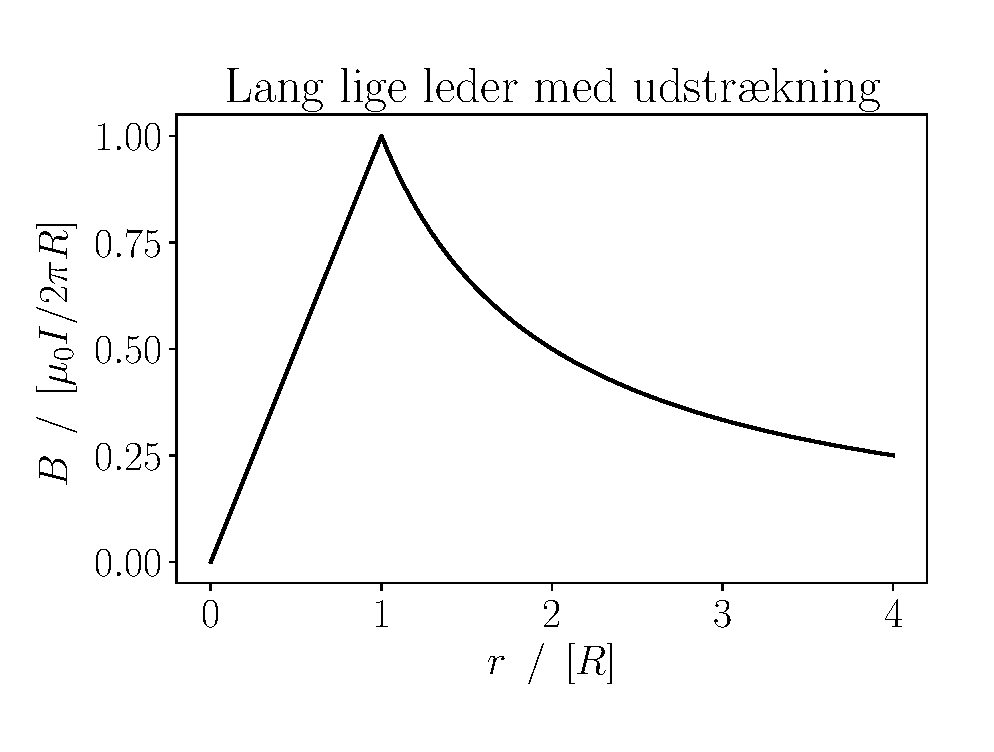
\includegraphics[width=\columnwidth]{Elektro/Elekfig/lange_lige_leder_cylinder.eps}
            \caption{Cylindrisk leder med radius $R$.}
            \label{fig:lang_lige_cylindrisk_leder}
        \end{subfigure}
        %
        \hfill
        %
        \begin{subfigure}[t]{.47\textwidth}
            \centering
            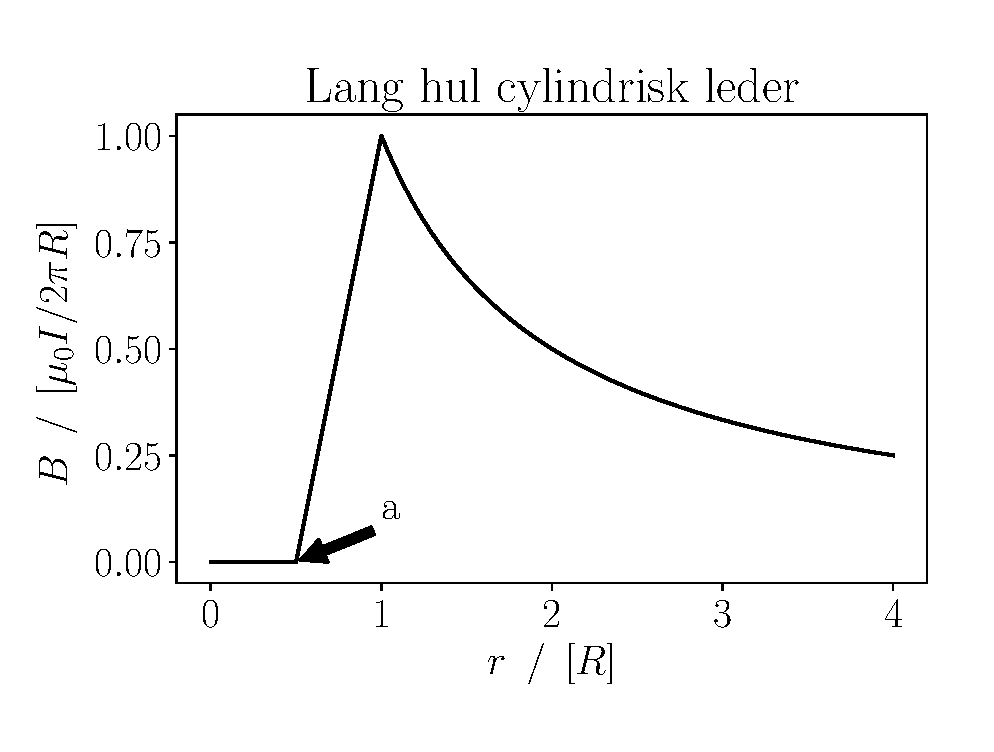
\includegraphics[width=\columnwidth]{Elektro/Elekfig/lange_lige_leder_hul_cylinder.eps}
            \caption{Hul cylindrisk leder med indre radius $a = R/2$ og ydre radius $R$.}
            \label{fig:lang_lige_hul_cylindrisk_leder}
        \end{subfigure}
        \caption{Størrelsen af af magnetfeltet for en lang lige leder med uniform strømfordeling som funktion af afstanden fra lederens centrum. Feltstyrken er angivet i enheder af den maksimale feltstyrke, $B(r/R)$.}
    \end{figure}
    %
    \opg Se figur \ref{fig:lang_lige_cylindrisk_leder}
    \opg Da cylinderen er hul med en indre radius $a$, løber der ingen strøm i området $r<a$. Ampereløkken kan vælges arbitræt indeni hulrummet uden at den vil indeslutte nogen strøm. For at opfylde Amperes lov må magnetfeltet derfor være nul i hulrummet og derfra har den samme form som for cylinderen uden hulrum, se figur \ref{fig:lang_lige_hul_cylindrisk_leder}.
\end{opgave}


\end{document}